\documentclass[12pt,table,xcdraw]{article}
\usepackage[utf8]{inputenc}



% Postavke za datum

\usepackage[ddmmyyyy]{datetime} % Format ddmmyyyy

% Slike i grafika

\usepackage[usenames,dvipsnames]{color} % Custom boje
\usepackage{graphicx} % Ubacivanje slika
\usepackage{tikz} % Crtanje
\usepackage{subfigure} 

% Matematika

\usepackage{amsmath,amsfonts,amsthm, mathtools} % Matematski paketi
\usepackage{amssymb} % Simboli
\usepackage{empheq} % Typesetting za math okruzenje
\usepackage{bm} % Bold za matematiku

% Programiranje

\usepackage{listings} % Ubacivanje progamskog koda
\usepackage[]{algorithm2e} % Pseudokodovi
\usepackage{courier} % font u listingu

% Header i Footer

\usepackage{fancyhdr} % Za editovanje headera
\usepackage{lastpage} % Da saznamo zadnju stranicu (za footer)
\usepackage{extramarks} % Za header i footer

% Hyperlinkovi

\usepackage[colorlinks = true,
            linkcolor = blue,
            urlcolor  = blue,
            citecolor=black
			]{hyperref} % da ToC moze da se klikce


% Naslovi i sekcije

\usepackage{titling} % Naslovi
\usepackage{sectsty} % Custom sekcije
\usepackage{caption} % Custom opcije za caption

% Tabele
\usepackage{multirow}


% Misc.

\usepackage{MnSymbol,wasysym} % ikonice
\usepackage{marvosym} % ikonice
\usepackage[alpine]{ifsym} % ikonice
\usepackage{lipsum} % Za placeholder text
\usepackage{verbatim} % Za begin i end comment naredbe
\usepackage{framed} % Okruzenje za okvir, shading, i leftline
\usepackage{float} % Floating (za sve)
\usepackage{changepage} % Za mijenjanje layouta stranice
\usepackage{varwidth} % Umjesto minipage
\usepackage[bottom]{footmisc} % fusnote
%\RequirePackage[no-math]{fontspec} % fontovi (samo za xelatex)
\usepackage[T1]{fontenc} % čćšđž za pdflatex
\usepackage[utf8]{inputenc} % utf 8 encoding

% BiBTeX logo
\usepackage{hologo} % Paketi
% Custom komande i redefinicije

\renewcommand{\contentsname}{Sadržaj} % Naslov ToC-a

\renewcommand{\dateseparator}{.} % Stavi tacku kao separator

\renewcommand{\algorithmcfname}{Algoritam} % Umjesto 'Algorithm'

\renewcommand{\figurename}{Slika} % Umjesto 'Figure'

\renewcommand{\tablename}{Tabela} % Umjesto 'Figure'

\renewcommand\refname{Reference} % Umjesto 'reference'

\newcommand{\cmark}{\ding{51}} % Checkmark
\newcommand{\xmark}{\ding{55}} % Xmark

\providecommand{\lxor}{\veebar} % Logicko XOR

\newcommand{\Z}{\mathbb{Z}} % Skup Z 

\setcounter{MaxMatrixCols}{15} % Vece matrice


% Margine
\topmargin=-0.45in
\evensidemargin=0in
\oddsidemargin=0in
\textwidth=6.5in
\textheight=9.0in
\headsep=0.25in

% CUSTOM KOMANDE:

\newcommand{\uokviri}[1]{ % Komanda koja nesto uokviri
\fbox{\begin{varwidth}{0.98\columnwidth}#1\end{varwidth}} 
}

\newcommand{\heart}{\ensuremath\varheartsuit} % srce

\newcommand{\linija}[1]{\rule{\linewidth}{#1}} % Custom naredba za horizontalnu liniju

% HEADER I FOOTER:

\pagestyle{fancy}
\lhead{} % Lijevi H
\chead{Data warehouse u bioskopu} % Centralni H
\rhead{\firstxmark} % Desni H
\lfoot{Elektrotehnički fakultet, Univerzitet u Sarajevu} % Lijevi F
\cfoot{} % Centralni F
\rfoot{Strana\ \thepage\ od\ \protect\pageref{LastPage}} % Desni F
\renewcommand\headrulewidth{0.4pt} % Velicina headera
\renewcommand\footrulewidth{0.4pt} % Velicina footera
 % Custom naredbe
% --------------------------------------------------------------------
% Definicije (ne mijenjaj)
% --------------------------------------------------------------------
\newcommand{\HRule}[1]{\rule{\linewidth}{#1}} 	

\makeatletter							% Naslov
\def\printtitle{%						
    {\centering \@title\par}}
\makeatother									

\makeatletter							% Autor
\def\printauthor{%					
    {\centering \large \@author}}				
\makeatother							

% --------------------------------------------------------------------
% Metapodaci (ovo treba mijenjati)
% --------------------------------------------------------------------
\title{	
		\normalsize \textsc{Univerzitet u Sarajevu}\\ 	
		\normalsize \textsc{Elektrotehnički Fakultet}\\ 	
		    \textsc{Stručni studij Razvoj Softvera}\\[4.0cm]
		 	\textsc{Skladišta podataka}\\		
			\LARGE \textbf{\uppercase{Data warehouse u bioskopu}}\\[2.0cm]	
		}

\author{
	    \rule{12cm}{0.3pt}\\[0.25cm]
        \Large Studenti:\\ % Umjesto ovoga mote i 'Autor' ako je jedan student a ne grupa
	Almir\textsc{Mulalić}, indeks \texttt{\#96-ST} \\
	Nađa \textsc{Alijagić}, indeks \texttt{\#69-ST} \\
	Alma \textsc{Feriz}, indeks \texttt{\#90-ST} \\
	Muhamed \textsc{Drinjak}, indeks \texttt{\#70-ST} \\
	Azra \textsc{Varnica}, indeks \texttt{\#50-ST} \\
       \rule{12cm}{0.3pt}\\[0.25cm]
              \vfill
        Predmetni profesor:\\
       Doc. dr Damir \textsc{Omerašević} dipl. el ing\\
        \vfill
        \today.\\ Sarajevo\\			% Danasnji datum
}

 % Naslovna stranica


\begin{document} 

\thispagestyle{empty}		% Bez numerisanja naslovne strane

\printtitle					% Ispisujemo naslov (komanda iz naslov_grupni.tex)

\printauthor				% Ispisujemo autora (komanda iz naslov_grupni.tex)

\newpage
\hypersetup{linkcolor=black}

\section{Uvod}

Razvojem informacijskih tehnologija i mogućnosti spremanja velikih količina podataka na disk javila se potreba za učinkovitim, strukturiranim načinima spremanja podataka tako da bi se mogli koristiti za analizu. Mnoge firme koriste sistem za skladištenja podataka kako bi poboljšale svoje poslovne procese i otkrile neke uzorke u ponašanju svojih korisnika. \\

DWH predstavlja bazu podataka koja omogućuje brzo i jednostavno izvoĎenje pretraga i upita nad velikim količinama podataka, kao i skup podataka na kojem se bazira sistem podrške u odlučivanju. Namijenjena je menadžerima, ali i svima koji u svom poslu obavljaju analitičke zadatke. Sadrži ogromne količine podataka, koji se koriste u svrhu poslovnih analiza i postizanja što boljih tržišnih rezultata. \\

U ovom radu ćemo detaljnije istražiti DWH u bioskopu.

\newpage

\section{UML reprezentacija relacijske baze podataka}

 Za modeliranje baza podataka i skladišta podataka mogu se koristiti UML-dijagrami klasa. Ključna prednost UML-a je intuitivnost upotrebe dijagrama i široka baza korisnika koji godinama rade s UML-dijagramima na najrazličitijim problemima oblikovanja sistema. U praktičnom dijelu rada izvedena je programska podrška koja omogućava automatsku izradu dimenzijskih relacija i činjenične relacije u relacijskoj bazi podataka na temelju konceptualnog modela skladišta definiranog UML-dijagramom klasa od strane korisnika-oblikovatelja skladišta podataka. \\
UML (Unified Modelling Language) služi za:
\begin{itemize}
\item Specifikaciju
\item Vizuelizaciju
\item Konstrukciju
\item Dokumentaciju razvoja softvera
\end{itemize}

\subsection{ER dijagram}

Model entiteta i veza nekog sistema, izražavamo preko entitete, atribute i veze pomoću dijagrama nazvanog ER dijagram
(Entity Relationship).
Velika prednost ER dijagrama jeste u tome što se lako crtaju i razumiju.
Dijagram sadrži tri osnovne konstrukcije:
\begin{itemize}
\item Entitete
\item Veze
\item Atribute
\end{itemize}


Na slici ispod se nalazi slika primjera ER dijagram kina. 

\newpage

\begin{figure}[h]
\centering
\captionsetup{justification=centering}
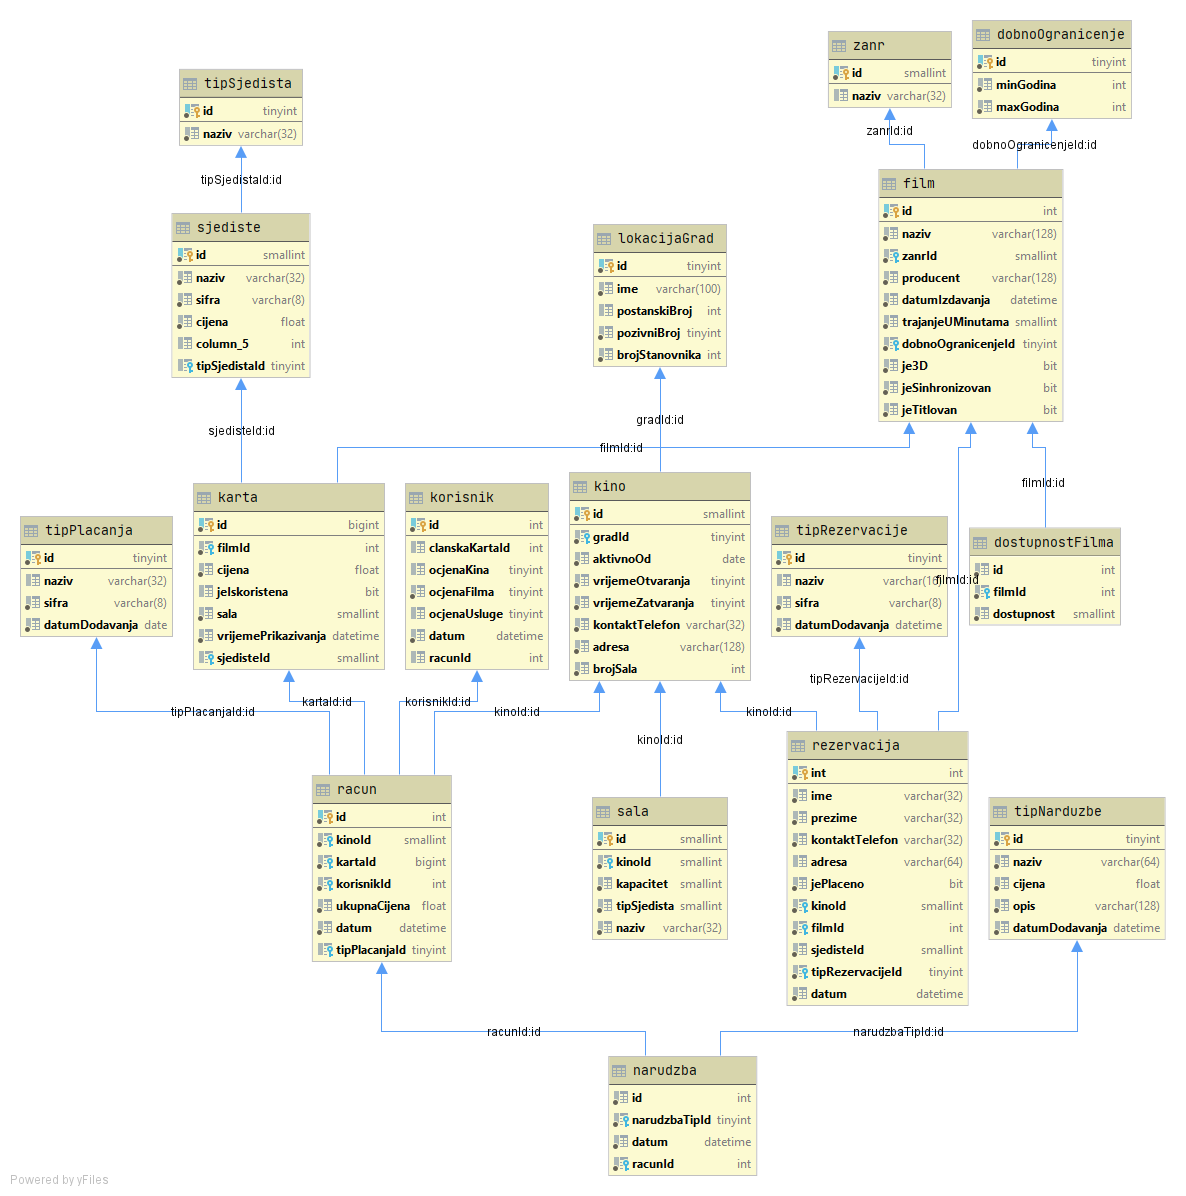
\includegraphics[width=0.85\columnwidth]{slike/slika1.png}
\label{fig:kod}
\end{figure}

\newpage

\subsection{Use case dijagram}

Dijagram slučajeva (engl. Use case diagram) prikaz je interakcije korisnika sa sistemom koji pokazuje odnos između korisnika i različitih slučajeva korištenja u kojima je korisnik uključen. Dijagram slučaja korišenja može indetifikovati različite tipove korisnika sistema i različite slučajeve korištenja i često će biti propraćen i drugim tipovima dijagrama. Slučajevi korištenja predstavljeni su krugovima ili elipsama.

\begin{figure}[h]
\centering
\captionsetup{justification=centering}
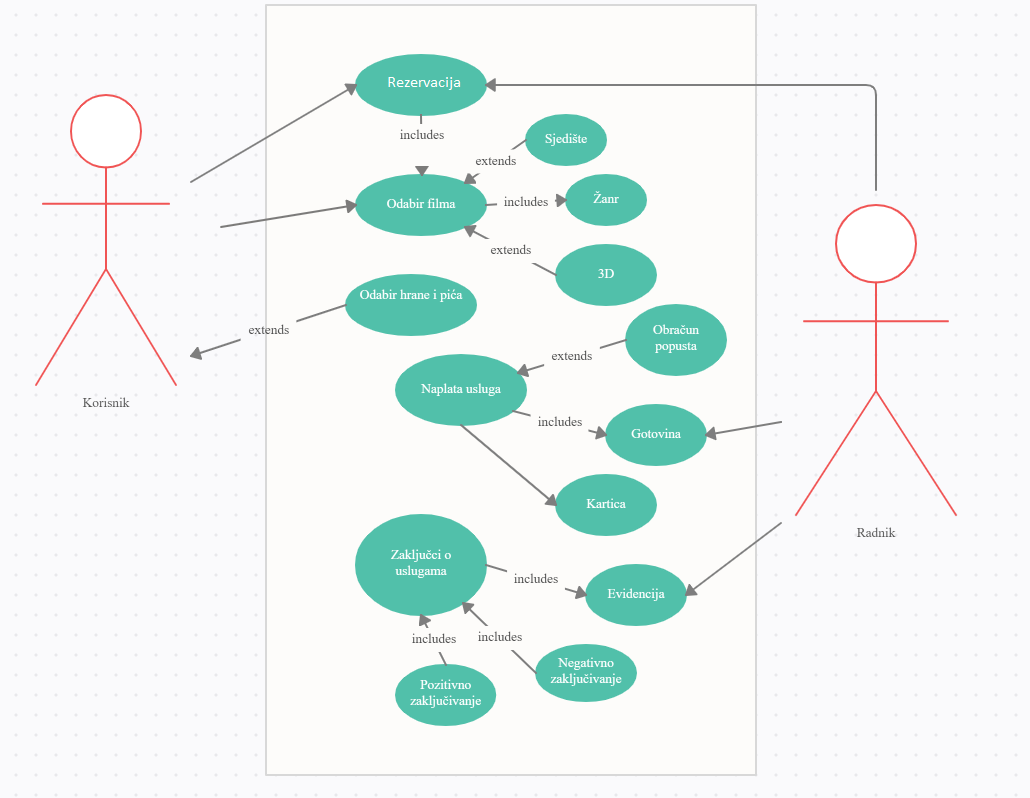
\includegraphics[width=0.85\columnwidth]{slike/slika4.png}
\label{fig:kod}
\end{figure}



\subsection{Dijagram aktivnosti}

Dijagram aktivnosti je dijagram koji ističe tok kontrole od aktivnosti do aktivnosti. Koristi se za prikaz tokova u sistemu, sa alternativnim putanjama. Sli
čan je klasičnim blok dijagramima, s tim što se na njemu prikazuju i paralelni tokovi. Aktivnost je ponašanje objekta dok je u određenom stanju. Tranzicija je kretanje od aktivnosti do aktivnosti ili od stanja do stanja. Služe za opis logike procedura, poslovnih postupaka i toka posla. Mogu prikazati i paralelna ponašanja. Pridružuju se klasi, odnosno njenoj operaciji ili slučaju korištenja.
\newpage

\begin{figure}[h]
\centering
\captionsetup{justification=centering}
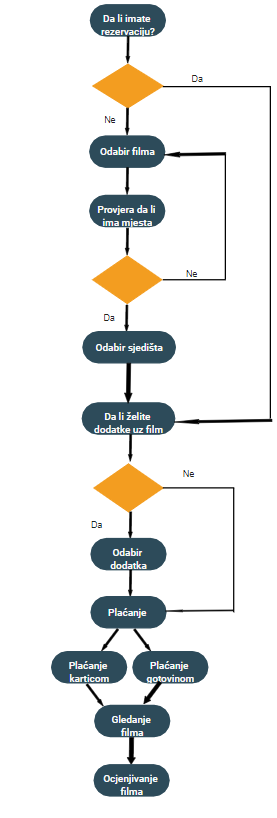
\includegraphics[width=0.35\columnwidth]{slike/slika2.png}
\label{fig:kod}
\end{figure}


\newpage
\subsection{Dijagram klasa}

Dijagram klasa (dio UML-a) jest vrsta strukturnog dijagrama u softverskom inžinjeringu, koji opisuje strukturu sustava objašnjavajući klase unutar sustava, njihove atribute i odnose.

\begin{figure}[h]
\centering
\captionsetup{justification=centering}
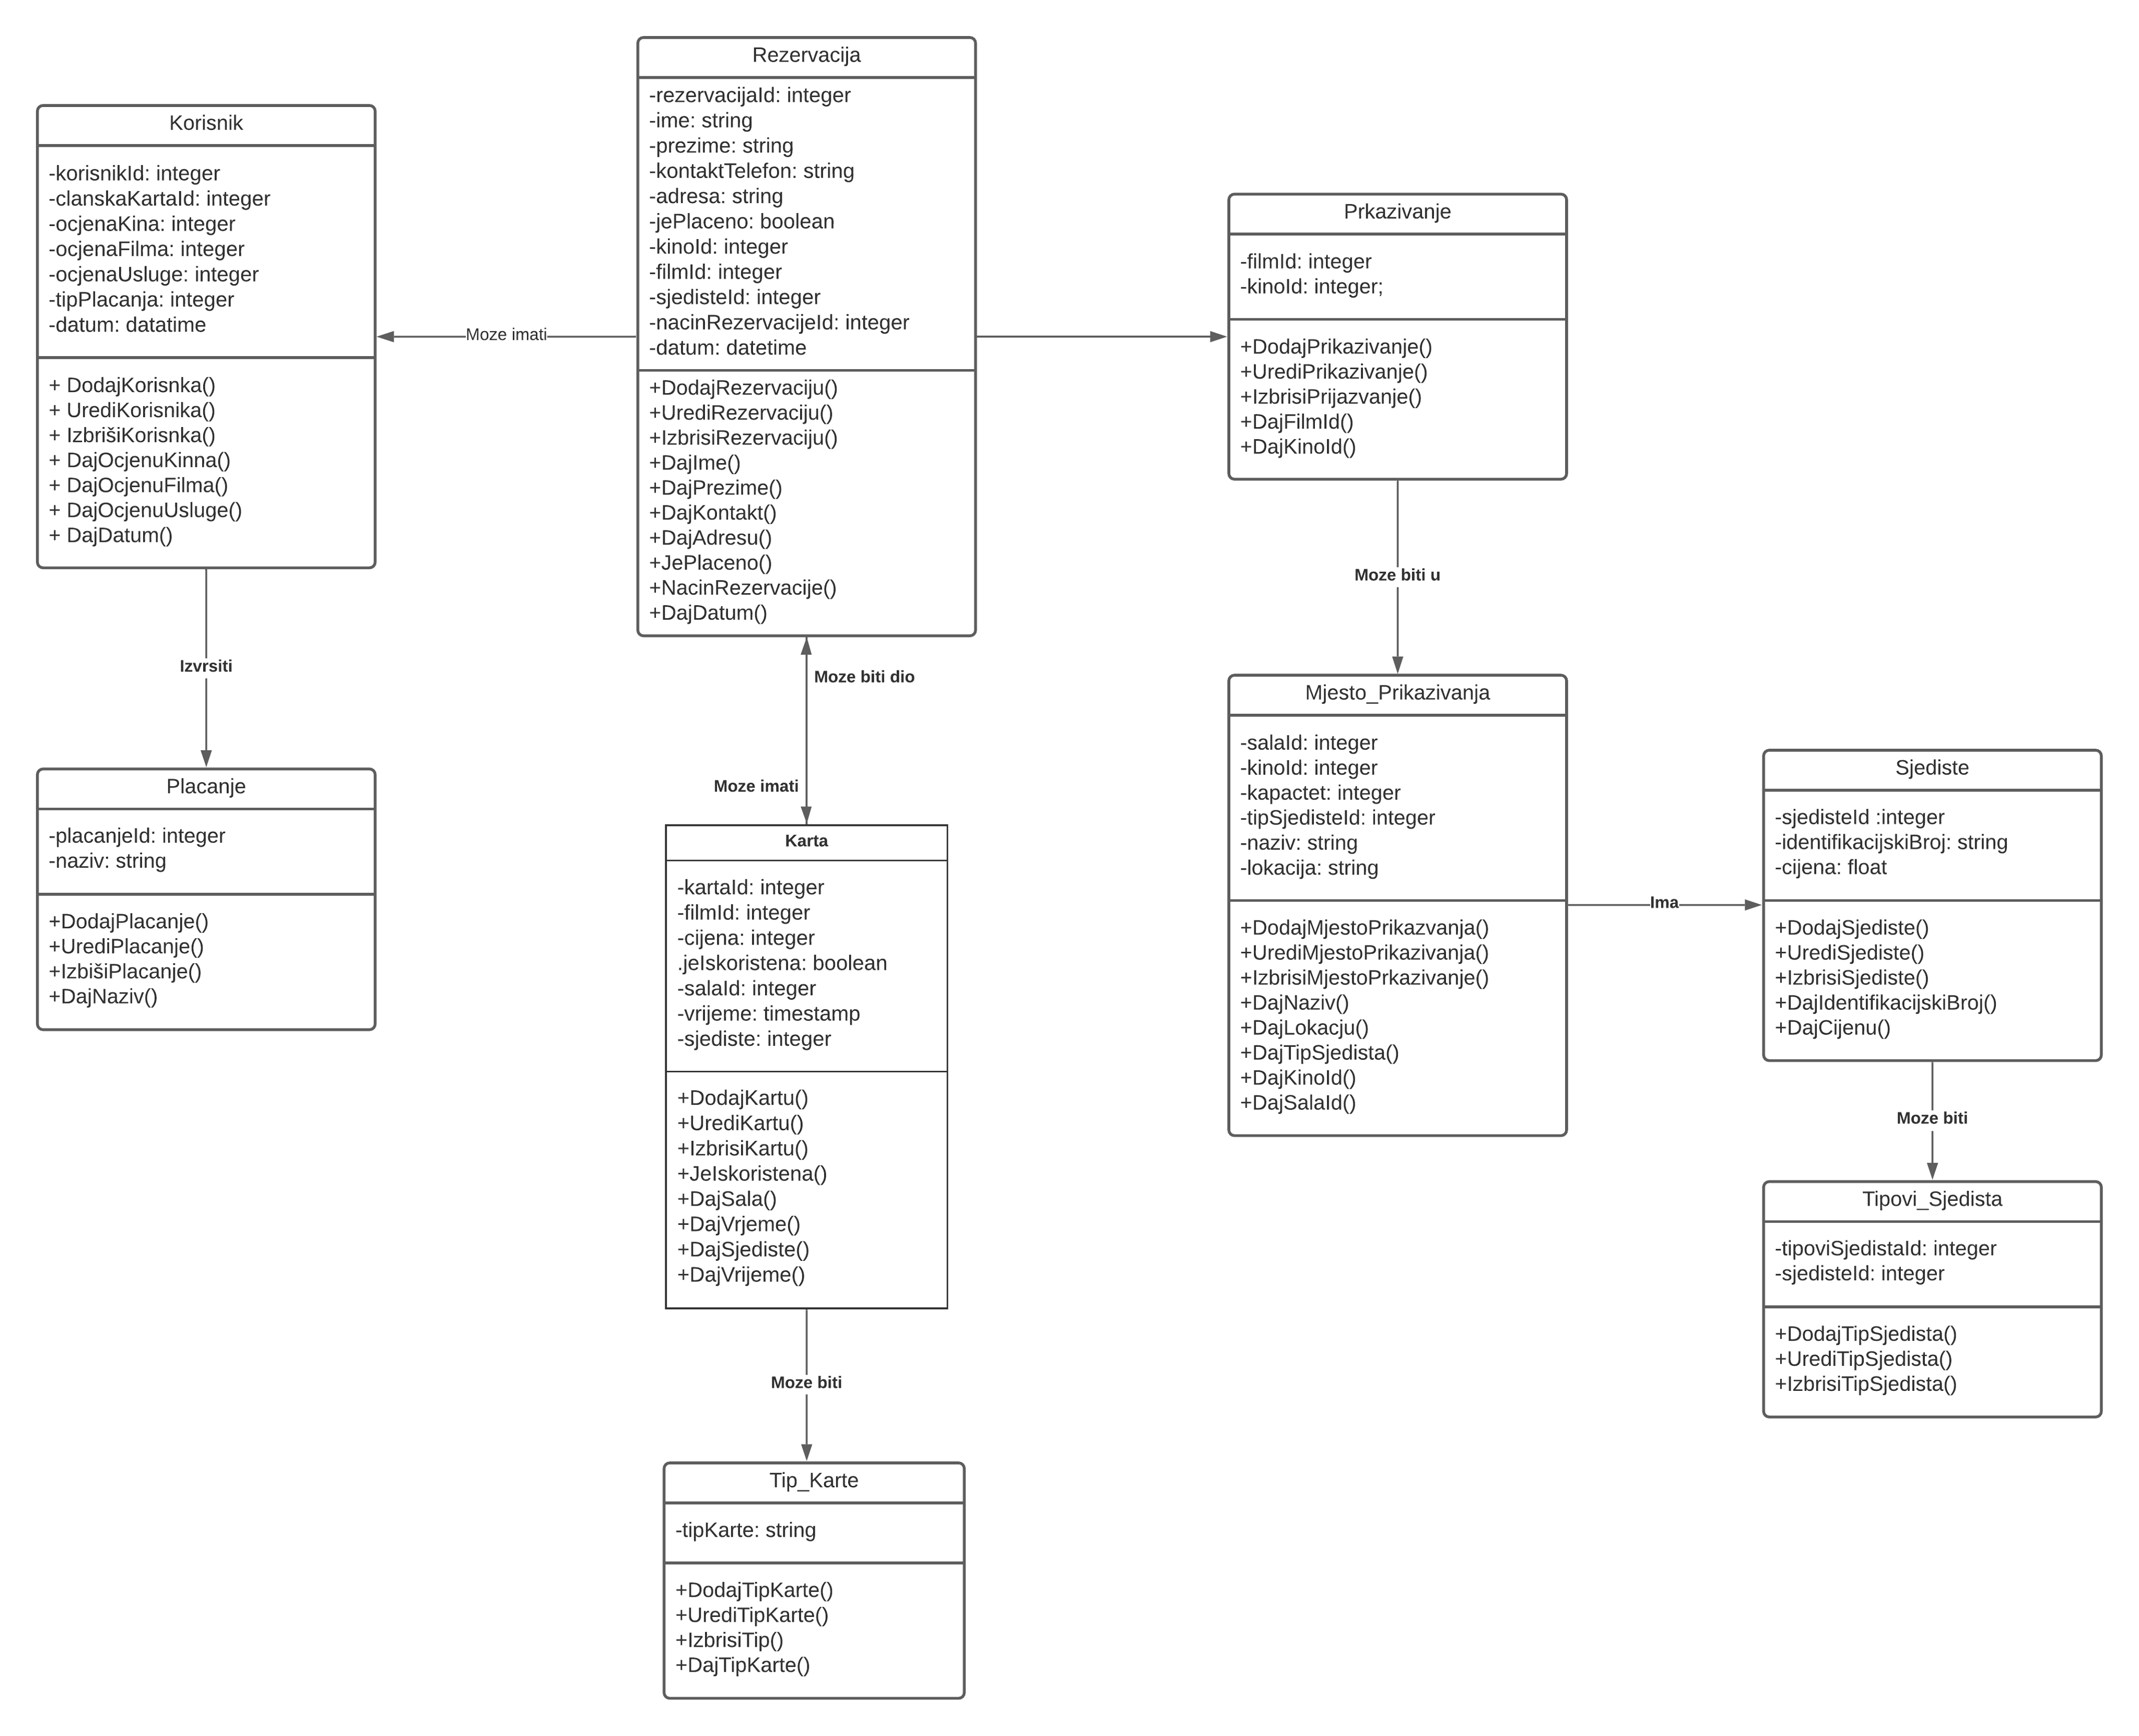
\includegraphics[width=0.85\columnwidth]{slike/slika3.png}
\label{fig:kod}
\end{figure}


\end{document}